\documentclass[11pt]{article}
\usepackage[margin=1in]{geometry}
\usepackage{graphicx}
\usepackage{amsmath}
\usepackage{subcaption}
\usepackage{booktabs}
\usepackage{hyperref}
\usepackage[numbers,sort&compress]{natbib}
\usepackage{lineno}
\usepackage{authblk}

\title{Nicotine-related beliefs induce dose-dependent responses in a thalamic circuit in human smokers}
\author[1]{Anonymous Submission}
\affil[1]{Target venue: \textit{Nature Human Behaviour}}
\date{}

\begin{document}
\maketitle

\begin{abstract}
Can a purely subjective belief act on the human brain with the graded precision of a pharmacological dose? We tested this by holding nicotine dose constant while parametrically manipulating instructed beliefs about the strength of an electronic cigarette. Twenty nicotine-dependent adult smokers (60 scans total) vaped a 1.2\% nicotine e-cigarette across three separate fMRI visits after being told, in a double-blind design, that the cartridge contained a ``low'', ``medium'' or ``high'' dose of nicotine; a non-smoking healthy-control group ($n=31$) was scanned on the same value-based investment task without vaping. Subjective perceived strength tracked the instructed label ($F(2,38)=9.71$, $P=0.0004$, partial $\eta^2=0.34$), whereas nicotine intake (mg), saliva cotinine and exhaled carbon monoxide were invariant across conditions ($P=0.178$, $0.393$, $0.698$). Value-related activity in the thalamus scaled parametrically with belief dose ($F(2,38)=3.62$, $P=0.036$; whole-brain cluster-level $P_\text{FWE}=0.006$, $k=50$), multivoxel patterns in the thalamus decoded belief condition at 49.3\% (chance 33.3\%, permutation $P=0.011$), and subjective perceived strength correlated with the thalamic signal across sessions (Spearman $r=0.27$, $P=0.035$). In contrast, the nucleus accumbens, putamen and caudate tracked reward overall but did not differentiate belief conditions. At the circuit level, thalamus-vmPFC functional coupling scaled with belief dose (cluster-level $P=0.041$ with small-volume correction). These data demonstrate that a cognitive construct---belief about a drug---can map onto a nAChR-rich thalamocortical circuit in a graded manner that quantitatively resembles pharmacological dose-response, with implications for placebo, personalized treatment, and the neural mechanisms of narrative influence in addiction.
\end{abstract}

\section{Introduction}

Human beliefs shape behavior and wellbeing, yet how a subjective mental construct is mapped onto neurobiological activity in a quantitatively graded fashion is largely unresolved. This gap is especially consequential for substance use disorders, where purely pharmacological accounts cannot explain the heterogeneity of drug response and the durability of craving after abstinence~\cite{picciotto2008nicotinic,benowitz2009pharmacology}. The placebo effect is the canonical case for belief-to-brain interaction: positive expectations about treatment can alter clinically meaningful outcomes and produce measurable shifts in neural activity even in the absence of active pharmacology~\cite{wager2004placebo,benedetti2013placebo}. Within addiction neuroscience, work with nicotine-dependent smokers has shown that binary beliefs about whether a cigarette contains nicotine selectively modulate reward prediction error signals in the ventral striatum~\cite{gu2015belief} and alter insular responses in deprived smokers~\cite{gu2016belief}. However, these demonstrations have been restricted to an all-or-none operationalization of belief, leaving open the question of whether beliefs can modulate neural activity with the graded precision that defines pharmacological dose-response relationships.

Pharmacology quantifies the impact of an agent through the dose-response function, in which the amount of active ingredient in a drug scales proportionally to a downstream biological readout. Nicotine in particular exerts well-characterized dose-dependent effects on regional brain activity measured with PET and functional MRI~\cite{brody2006cigarette,cosgrove2009beta2}. The thalamus is an especially informative locus in this regard: it harbors one of the highest densities of nicotinic acetylcholine receptors (nAChRs) in the human brain~\cite{picciotto2008nicotinic,cosgrove2009beta2}, and its activity has been shown to scale with nicotine exposure~\cite{brody2006cigarette}. At the same time, PET imaging has shown that smoking denicotinized or low-nicotine-content cigarettes is sufficient to occupy a substantial fraction of nAChRs in the human brain~\cite{brody2011ventral,cosgrove2009beta2}, implying that factors beyond raw nicotine dose---plausibly including expectations, habits, and beliefs about the act of smoking---shape receptor-level readouts.

We reasoned that if subjective beliefs about a drug can act on the brain with quantitative precision, then an experimental manipulation that holds actual nicotine dose constant while parametrically varying the instructed belief about the dose should yield graded, dose-like neural responses in thalamic circuitry. To test this, we instructed 20 nicotine-dependent human smokers (60 fMRI scans in total) across three visits that an e-cigarette they were about to vape contained ``low'', ``medium'', or ``high'' levels of nicotine, while actual nicotine content was held constant at 1.2\% across all cartridges. After vaping, participants performed a value-based investment task during fMRI. A non-smoking healthy-control group ($n=31$) was scanned on the same task without vaping and was used as a reference. We chose e-cigarettes as the delivery vehicle because they permit finer control over nicotine strength than traditional cigarettes and because smokers in our sample were naive to vaping, reducing conditioned cue effects that have been proposed to drive striatal responses in prior belief-by-drug experiments~\cite{gu2015belief}.

Our predictions were grounded in the anatomical and pharmacological properties of thalamocortical circuits. Because the thalamus gates sensory and value-related information and is densely innervated by nAChRs~\cite{sherman2016thalamus,halassa2017thalamic}, we hypothesized that value-related thalamic activity would scale parametrically with instructed belief dose. We further predicted that thalamocortical coupling with the ventromedial prefrontal cortex (vmPFC)---a region repeatedly linked to value representation~\cite{plassmann2007orbitofrontal,levy2012root}, task-state encoding~\cite{wilson2014orbitofrontal,schuck2016human}, and belief-related inference~\cite{rouault2018belief,rouault2022prefrontal}---would likewise track belief dosage. In contrast, we expected that the ventral striatum, which is strongly shaped by conditioned cigarette cues and reinforcement history~\cite{haber2010reward,schultz1997neural,kober2010brain}, would track reward value overall but would not differentiate between belief conditions in a cohort unfamiliar with the delivery device.

\section{Related Work}

\paragraph{Beliefs and the brain in addiction.} Prior work established that telling smokers a cigarette contained or did not contain nicotine selectively shifted striatal value-learning signals despite identical pharmacology~\cite{gu2015belief}. A follow-up study showed that the same manipulation altered insular activity and subjective craving in abstinent smokers~\cite{gu2016belief}. These studies framed belief as a binary factor (nicotine present vs. absent). Our design extends this line of work by introducing a three-level dose manipulation and by probing thalamic rather than only striatal circuitry.

\paragraph{Dose-response imaging of nicotine.} Pharmacological imaging has established dose-dependent thalamic and striatal effects of nicotine itself~\cite{brody2006cigarette,brody2011ventral,cosgrove2009beta2}. Across these studies, the thalamus has emerged as the region most reliably tracking nicotine exposure, consistent with its high nAChR density~\cite{picciotto2008nicotinic}. Our study asks the complementary question: whether a purely cognitive manipulation can produce an analogous graded effect in the same anatomical substrate.

\paragraph{Placebo and expectation.} Expectation-based placebo effects recruit a distributed circuitry including prefrontal, striatal, and brainstem regions~\cite{wager2004placebo,benedetti2013placebo}. Most placebo experiments contrast an active and an inactive condition, leaving unclear whether expectation acts on the brain with pharmacological-style precision. We bring the dose-response logic of pharmacology into the placebo tradition by using three graded levels of instructed strength.

\paragraph{Value, state, and belief in vmPFC.} The vmPFC encodes subjective value across reward modalities~\cite{plassmann2007orbitofrontal,levy2012root} and represents abstract task states~\cite{wilson2014orbitofrontal,schuck2016human}. Recent work has shown that the vmPFC participates in self-performance estimation and belief updating~\cite{rouault2018belief,rouault2022prefrontal}. These findings motivate our focus on thalamocortical coupling with vmPFC as the circuit most likely to carry parametric belief signals.

\paragraph{Thalamus in cognition.} The thalamus is now appreciated as more than a passive relay: it contributes actively to cortical computation and cognitive control~\cite{sherman2016thalamus,halassa2017thalamic}. Its role in gating incoming information makes it a plausible substrate for belief-driven dose-like modulation, particularly given its nAChR density~\cite{picciotto2008nicotinic}.

\paragraph{Methodological substrate.} For atlas-based ROI definition we used the WFU Pick Atlas~\cite{maldjian2003automated} and the THOMAS thalamic parcellation~\cite{mcleod2017spatially}. Motion artefact was mitigated with ArtRepair~\cite{mazaika2009artifact}, and connectivity was evaluated with psychophysiological interaction analysis~\cite{friston1997psychophysiological}. Participant characterization used the Fagerstr\"{o}m Test for Nicotine Dependence~\cite{fagerstrom1991measuring} and companion substance-use questionnaires.

\section{Results}

\subsection{Instructed beliefs modulated subjective perception without shifting pharmacology}

Our experimental manipulation relied on a three-visit, within-subject design in which identical 1.2\% nicotine e-cigarette cartridges were relabelled as ``low'', ``medium'' or ``high''. After a 20-minute vaping period on each visit, participants rated the perceived strength of the nicotine on a 10-point scale and then performed a value-based investment task during fMRI (see Methods and Fig.~\ref{fig:fig1}). Subjective ratings scaled monotonically with the instructed label: low $=3.52 \pm 0.61$, medium $=4.52 \pm 0.41$, high $=5.82 \pm 0.47$ (mean $\pm$ SD in arbitrary units), yielding a repeated-measures ANOVA $F(2,38)=9.71$, $P=0.0004$, partial $\eta^2=0.34$ (90\% CI: $0.12 \leq \eta^2 \leq 0.48$). This effect confirms that the instruction modified the perceived strength of nicotine across visits in our smoker sample.

Three converging sanity checks ensured that the belief manipulation did not confound actual pharmacology. First, nicotine intake, computed from the change in cartridge weight multiplied by the nominal 1.2\% nicotine content, did not differ across conditions (low $=0.928 \pm 0.56$, medium $=0.719 \pm 0.423$, high $=0.783 \pm 0.434$ mg; $F(2,38)=1.806$, $P=0.178$). Second, vaping-induced changes in saliva cotinine---the principal nicotine metabolite, quantified by a validated LC-MS/MS method with d$_3$-cotinine internal standard---were comparable between conditions ($F(2,32)=0.959$, $P=0.393$). Third, exhaled carbon monoxide measured before vaping, which indexes baseline nicotine saturation, was likewise invariant ($F(2,32)=0.364$, $P=0.698$). The mean consumed nicotine ($\sim0.8$ mg per session) was in the same range as traditional cigarette exposures used in our prior work and in the nicotine-imaging literature~\cite{brody2006cigarette,gu2015belief}. Taken together, these checks confirm that any downstream neural differences between conditions cannot be attributed to consumed nicotine, metabolism, or baseline saturation.

\begin{figure}[t]
  \centering
  \begin{subfigure}{0.48\linewidth}
    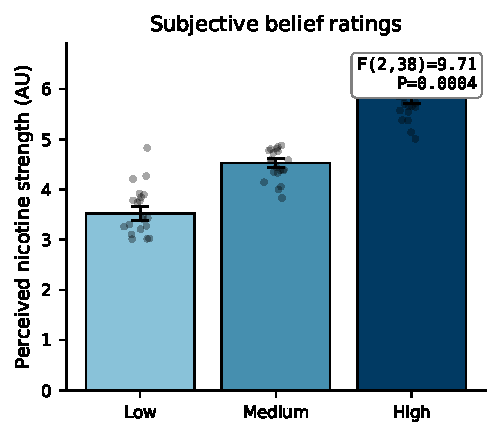
\includegraphics[width=\linewidth]{figures/fig1b_belief_ratings.pdf}
    \caption{}
    \label{fig:belief-ratings}
  \end{subfigure}\hfill
  \begin{subfigure}{0.48\linewidth}
    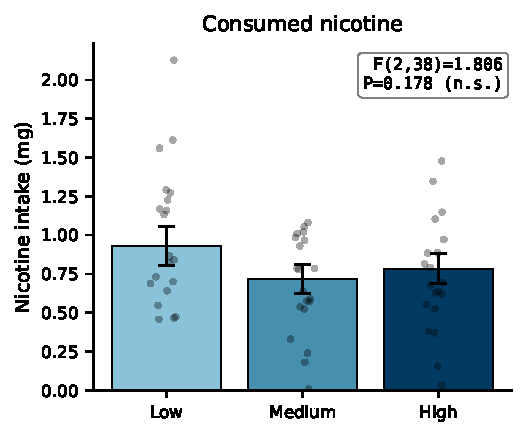
\includegraphics[width=\linewidth]{figures/fig1c_nicotine_intake.pdf}
    \caption{}
    \label{fig:nicotine-intake}
  \end{subfigure}
  \caption{\textbf{Belief manipulation and sanity checks.} (\subref{fig:belief-ratings}) Subjective perceived nicotine strength scales with the instructed label (low $3.52 \pm 0.61$, medium $4.52 \pm 0.41$, high $5.82 \pm 0.47$ AU; rmANOVA $F(2,38)=9.71$, $P=0.0004$, partial $\eta^2=0.34$). (\subref{fig:nicotine-intake}) Consumed nicotine does not differ across belief conditions (low $0.928 \pm 0.56$, medium $0.719 \pm 0.423$, high $0.783 \pm 0.434$ mg; $F(2,38)=1.806$, $P=0.178$). Cotinine and exhaled carbon monoxide are similarly invariant across conditions ($P=0.393$ and $P=0.698$; not shown). Bars, group means; points, participants; error bars, SEM.}
  \label{fig:fig1}
\end{figure}

\begin{figure}[t]
  \centering
  \begin{subfigure}{0.49\linewidth}
    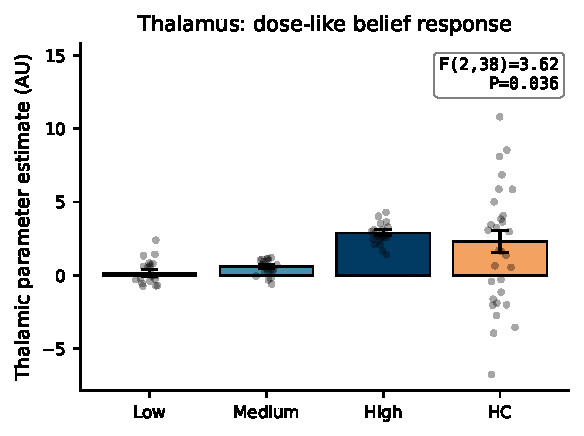
\includegraphics[width=\linewidth]{figures/fig2b_thalamus_bars.pdf}
    \caption{}
    \label{fig:thalamus-bars}
  \end{subfigure}\hfill
  \begin{subfigure}{0.49\linewidth}
    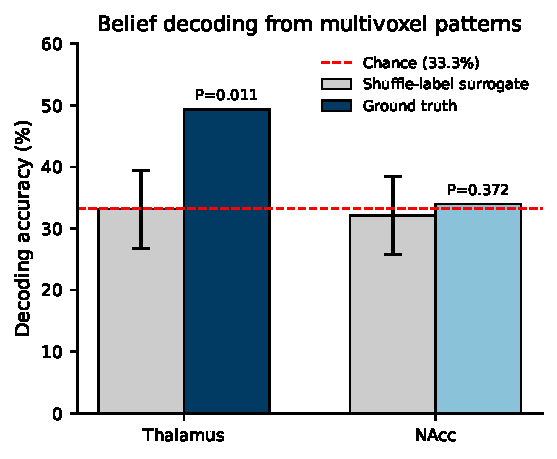
\includegraphics[width=\linewidth]{figures/fig2d_decoding.pdf}
    \caption{}
    \label{fig:decoding}
  \end{subfigure}
  \caption{\textbf{Thalamic activity encodes a dose-like belief signal.} (\subref{fig:thalamus-bars}) Value-tracking parameter estimates in an independent thalamic ROI scale parametrically with instructed belief (low $0.157 \pm 1.047$, medium $0.601 \pm 0.714$, high $2.914 \pm 0.865$ AU; rmANOVA $F(2,38)=3.62$, $P=0.036$, partial $\eta^2=0.16$). Non-smoking healthy controls (HC, $n=31$, $2.318 \pm 4.258$ AU) do not differ significantly from any single smoker condition (two-sample $t$-tests, all $P>0.05$). (\subref{fig:decoding}) Multivoxel decoding of belief condition from thalamic patterns reaches 49.3\% (chance 33.3\%, shuffle-label surrogate $33.1 \pm 6.3$\%, $P=0.011$), whereas decoding from nucleus accumbens patterns is at 34.0\% (surrogate $32.1 \pm 6.3$\%, $P=0.372$). Bars, means; error bars, SEM or shuffle surrogate SD.}
  \label{fig:fig2}
\end{figure}

\begin{figure}[t]
  \centering
  \begin{subfigure}{0.49\linewidth}
    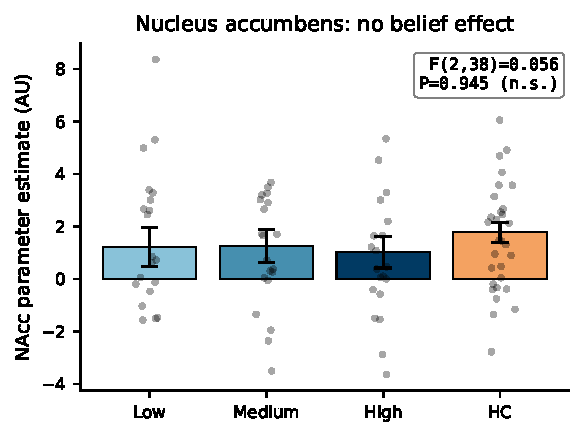
\includegraphics[width=\linewidth]{figures/fig3b_nacc_bars.pdf}
    \caption{}
    \label{fig:nacc-bars}
  \end{subfigure}\hfill
  \begin{subfigure}{0.49\linewidth}
    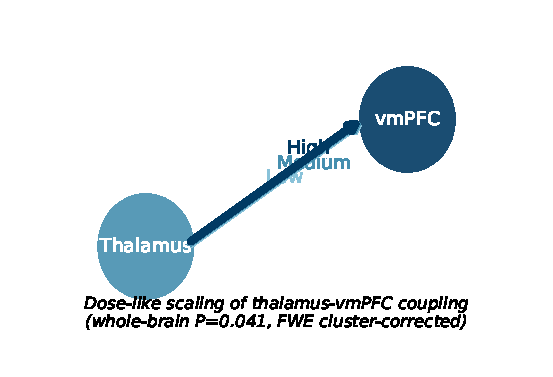
\includegraphics[width=\linewidth]{figures/fig4_ppi_schematic.pdf}
    \caption{}
    \label{fig:ppi-schematic}
  \end{subfigure}
  \caption{\textbf{Negative striatal result and thalamus-vmPFC coupling.} (\subref{fig:nacc-bars}) Nucleus accumbens parameter estimates do not differentiate belief conditions (smokers low $1.228 \pm 3.329$, medium $1.248 \pm 2.828$, high $1.016 \pm 2.6983$ AU; rmANOVA $F(2,38)=0.056$, $P=0.945$) and are comparable to HC ($1.781 \pm 2.138$ AU; all between-group $t$-tests $P>0.25$). Putamen and caudate also show no belief effect ($P=0.327$ and $P=0.781$). (\subref{fig:ppi-schematic}) Schematic of the key psychophysiological-interaction finding: functional coupling between the thalamus and vmPFC scales with belief dose (whole-brain $P=0.041$, FWE cluster-corrected at cluster-defining $P<0.005$, $k=50$).}
  \label{fig:fig3}
\end{figure}

\subsection{Thalamic value signals tracked belief dose parametrically}

We next asked how beliefs mapped onto neural activity during the investment task. Each trial $t$ involved a bet $b_t$ informed by recent market history; the absolute fractional return $|r_t| = |(p_t - p_{t-1})/p_{t-1}|$ served as the magnitude of attainable reward, used as the key parametric modulator in a whole-brain GLM. A second-level random-effects repeated-measures ANOVA with belief as the main factor (``low'', ``medium'', ``high'') identified a single cluster in which value-tracking activity scaled parametrically with belief dose: the left thalamus (peak at MNI $(-15, -19, -1)$, cluster-level $P_\text{FWE}=0.006$, cluster-defining $P<0.005$ uncorrected, extent $k=50$). No other region survived the same threshold at the whole-brain level.

An ROI analysis using an independent anatomical thalamus mask~\cite{maldjian2003automated} corroborated this effect (Fig.~\ref{fig:fig2}a). Parameter estimates increased with belief (low $=0.157 \pm 1.047$, medium $=0.601 \pm 0.714$, high $=2.914 \pm 0.865$ AU; $F(2,38)=3.62$, $P=0.036$, partial $\eta^2=0.16$, 90\% CI: $0.006 \leq \eta^2 \leq 0.30$). These thalamic activations did not differ significantly from those of non-smoking healthy controls ($\mathrm{HC} = 2.318 \pm 4.258$ AU; smokers-low vs HC $t(49)=1.95$, $P=0.057$; smokers-medium vs HC $t(49)=1.53$, $P=0.132$; smokers-high vs HC $t(49)=-0.50$, $P=0.616$), indicating that the strongest belief condition brought thalamic value-tracking in smokers into a range indistinguishable from that of unexposed controls performing the identical task.

To guard against assumptions about the null distribution, we also ran a non-parametric permutation analysis in which belief labels were shuffled within participant (preserving one label per condition per subject). Beta estimates for the true label allocation ranked significantly higher than the surrogate distribution ($N=1{,}000$, $P=0.002$), providing a label-permutation-based confirmation of the rmANOVA result. A finer parcellation of the thalamus using the THOMAS atlas~\cite{mcleod2017spatially} localized the effect predominantly to ventral posterior nuclei---centromedian (CM) and lateral geniculate (LGN)---with VPL, pulvinar, LGN and CM all surviving FDR correction at $q=0.05$ (Supplementary Fig.~S2).

We then asked whether belief condition could be \textit{decoded} from distributed thalamic voxel patterns using a regularized linear discriminant analysis (rLDA) classifier with 10-fold cross-validation (see Methods). The classifier achieved 49.3\% classification accuracy, significantly above the chance level of 33.3\%; a shuffled-label permutation test ($N=10{,}000$) yielded a surrogate distribution of $33.1 \pm 6.3$\%, $P=0.011$ (Fig.~\ref{fig:fig2}b). Within the THOMAS sub-nuclei, only the ventral posterolateral nucleus survived FDR correction ($P=0.018$).

Belief effects on the thalamus were not merely group-level: they also tracked individual variability in the subjective experience of nicotine strength. Across all 60 sessions, self-reported perceived strength correlated with the thalamic reward parameter estimate (Spearman $r=0.27$, $P=0.035$), linking neural dose-response to perceptual dose-response within individuals.

Finally, we verified that the thalamic effect was not driven by low-level confounds. Regressors modeling button presses (motor) and market viewing (visual) revealed no differential thalamic engagement across belief conditions (Supplementary Fig.~S3a). Re-running the pipeline without spatial smoothing reproduced the belief-graded thalamic effect (Supplementary Fig.~S3b), ruling out preprocessing artefacts as an alternative explanation.

\subsection{Striatal reward tracking was invariant to belief}

A previous study using an analogous design but with traditional cigarettes showed that a binary belief manipulation shifted ventral striatal prediction-error signals~\cite{gu2015belief}. Motivated by that result, we analyzed the striatum as a pre-registered contrast. Consistent with a large reward-processing literature~\cite{haber2010reward,schultz1997neural}, the ventral striatum tracked the market value signal $|r_t|$ in the pooled cross-condition contrast ($P_\text{FDR} < 0.01$; Supplementary Fig.~S4a). However, striatal reward responses did not differ across belief conditions at the whole-brain level ($P>0.05$, Supplementary Fig.~S5a).

Consistent with the whole-brain null, an ROI analysis on an independent nucleus accumbens (NAcc) mask showed no belief effect (smokers low $=1.228 \pm 3.329$, medium $=1.248 \pm 2.828$, high $=1.016 \pm 2.6983$ AU; $F(2,38)=0.056$, $P=0.945$; permutation $P=0.94$; Fig.~\ref{fig:fig3}a). NAcc activations were statistically comparable to healthy controls ($\mathrm{HC}=1.781 \pm 2.138$ AU; all between-group $t$-tests $P>0.25$). Multivariate decoding of belief from NAcc voxel patterns was not significant (ground truth 34.0\%, surrogate $32.1 \pm 6.3$\%, $P=0.372$; also reported in Fig.~\ref{fig:fig2}b). Neither the putamen ($F(2,38)=1.15$, $P=0.327$) nor the caudate ($F(2,38)=0.24$, $P=0.781$) showed a belief effect.

The lack of a striatal effect was consistent with the absence of a belief-by-return interaction in participants' choice behavior (Supplementary Information and Supplementary Table~S1), suggesting that in this study the experimentally induced belief did not permeate reinforcement-learning updates. One plausible account is that smokers were naive to vaping and therefore lacked the pre-established sensory associations that traditional cigarettes carry for chronic smokers.

\subsection{Belief modulated thalamus-vmPFC functional coupling}

To ask whether belief dose-response propagated along thalamocortical circuits, we conducted a psychophysiological-interaction (PPI) analysis~\cite{friston1997psychophysiological} using the bilateral thalamus as the seed and market reveal as the psychological context. In a second-level rmANOVA across belief conditions, the thalamus-vmPFC coupling showed a dose-dependent effect at the whole-brain level (cluster-level $P=0.041$ with small-volume correction over the vmPFC, FWE cluster-corrected at cluster-defining $P<0.005$). An independent 6-mm spherical ROI centred on a vmPFC coordinate derived from a prior belief-formation study~\cite{rouault2018belief} confirmed the effect (peak MNI $(-11, 50, -6)$; Supplementary Fig.~S7a; schematic in Fig.~\ref{fig:fig3}b). In sharp contrast, a PPI with the ventral striatum as seed did not yield significant belief-graded connectivity to vmPFC or elsewhere at the same threshold, reinforcing the specificity of the thalamic result.

Taken together, the ROI, whole-brain, decoding, permutation and PPI analyses converge on a single conclusion: the thalamus and its projection to vmPFC carry a graded neural signature of belief dose, whereas canonical mesolimbic reward regions do not differentiate between belief conditions in this vaping-naive cohort.

\section{Discussion}

\paragraph{Summary of findings.} We asked whether a purely cognitive construct---belief about the strength of a drug---can act on the human brain in a quantitatively graded fashion analogous to a pharmacological dose-response. Using a within-subject design in which 20 nicotine-dependent smokers were scanned three times after vaping e-cigarettes whose labels (``low'', ``medium'', ``high'') were manipulated despite an invariant 1.2\% nicotine content, we observed three convergent belief effects. First, subjective perceived strength tracked the instructed label despite no change in nicotine intake, cotinine metabolism or carbon monoxide saturation. Second, value-related activity in the thalamus---measured with a whole-brain GLM, an independent anatomical ROI, a non-parametric permutation test, and a regularized linear discriminant decoder---scaled parametrically with belief dose, and correlated within individuals with subjective perceived strength. Third, thalamic-vmPFC functional connectivity also scaled with belief dose. The ventral striatum tracked reward overall but did not distinguish belief conditions. The central claim is therefore not about average pharmacology, but about the \textit{shape} of the belief-to-brain mapping: in a nAChR-rich thalamocortical circuit, subjective belief behaves like a graded dose.

\paragraph{Why the thalamus.} The thalamus is a particularly plausible substrate for belief dose-response. It contains one of the highest densities of $\alpha_4\beta_2$ nAChRs in the human brain~\cite{picciotto2008nicotinic,cosgrove2009beta2}, and its activity scales with nicotine exposure in PET and fMRI~\cite{brody2006cigarette,brody2011ventral}. Crucially, the PET literature already forced a puzzle onto the field: smokers who consume denicotinized or low-nicotine cigarettes still exhibit a substantial fraction of nAChR occupancy~\cite{brody2011ventral,cosgrove2009beta2}, and even second-hand smoke produces measurable occupancy~\cite{cosgrove2009beta2}. Pharmacology alone cannot account for this gap. Our findings supply one component of a candidate mechanism: the beliefs and expectations a smoker holds about a smoking act can drive graded activation in the same thalamic substrate that nicotine itself engages. Expressed differently, our result reframes the thalamus from a node whose activity scales with the chemical quantity of nicotine to a node whose activity scales with the \textit{represented} dose, with pharmacology and belief acting as two inputs into a common graded readout. The anatomical specificity observed (CM, LGN, VPL and pulvinar) also fits a broader role of the thalamus as an active participant in cortical computation and attention rather than a passive relay~\cite{sherman2016thalamus,halassa2017thalamic}, and resonates with work showing that thalamic nuclei gate the propagation of task-relevant information.

\paragraph{vmPFC as a dosing partner.} The parametric scaling of thalamus-vmPFC coupling is the circuit-level counterpart of the regional effect. The vmPFC encodes a common currency of subjective value~\cite{plassmann2007orbitofrontal,levy2012root}, represents task states~\cite{wilson2014orbitofrontal,schuck2016human}, and is implicated in belief-related inference and metacognition~\cite{rouault2018belief,rouault2022prefrontal}. Earlier work documented a binary role for belief in gating thalamocortical interactions. Our data extend this by showing that the vmPFC-thalamus circuit encodes belief parametrically rather than as an on/off switch, a distinction of considerable theoretical interest because it renders ``belief'' measurable in units that are commensurate with pharmacology. The circuit-level result is also methodologically robust: the effect survives both whole-brain cluster correction with small-volume correction in vmPFC and an independent vmPFC ROI drawn from a prior belief-formation study~\cite{rouault2018belief}, and it is specific to thalamic rather than striatal seeds.

\paragraph{Reconciling the striatum null with prior work.} A previous study with a similar factorial design reported that the ventral striatum tracked binary belief about whether a cigarette contained nicotine~\cite{gu2015belief}. Our study does not replicate that particular striatal effect, despite a conceptually related design. We view this divergence as informative rather than inconsistent. Three design features matter. First, smokers in our sample were naive to e-cigarettes, whereas the prior study used the smokers' habitual delivery device. The striatum is known to be sensitive to conditioned reward cues~\cite{haber2010reward,kober2010brain}; stripping the conditioned context may remove the very signal on which a striatal belief effect would ride. Second, mean consumed nicotine was higher here ($\sim0.8$ mg per session) than in the prior study ($\sim0.6$ mg). Because the thalamus hosts a higher density of nAChRs than the striatum, the thalamus is more likely to dominate the pharmacological readout at this higher dose, whereas the striatum may be saturated or decoupled from the pharmacological gradient at this level. Third, our three-level dose design probes graded encoding rather than the binary presence/absence contrast of the prior work. Put together, the pattern suggests that striatal and thalamic belief effects occupy complementary regimes: the striatum is sensitive to conditioned binary belief in habitual contexts, whereas the thalamus encodes graded belief dose even without conditioning.

\paragraph{Implications for addiction, placebo, and mental health.} The practical interest of a quantitatively graded belief-to-brain mapping is that it turns belief into a handle that is potentially titratable alongside pharmacology. Placebo experiments have long shown that expectation alters brain activity~\cite{wager2004placebo,benedetti2013placebo}. What has been harder to demonstrate is that expectation acts on neurobiology in the same quantitative coordinate system as a drug. Our findings bring this demonstration into the addiction domain for the first time, and they do so in the very circuit that carries the drug's pharmacological signal. The immediate consequence is that heterogeneity in pharmacological response---a long-standing clinical puzzle for smoking cessation and for psychiatric treatment more generally---can in principle be decomposed into a pharmacological component and a belief component, with the thalamus as a candidate substrate for the latter. More broadly, our results motivate the development of interventions that deliberately shape patients' narratives about their medications, and provide a measurable neural target against which such interventions could be evaluated.

\paragraph{Limitations.} Four caveats warrant emphasis. First, the smoker sample is modest ($n=20$ with 60 scans), reflecting a power calculation based on a previous effect size ($d=0.69$) rather than an oversized confirmatory sample; replication in a larger cohort remains necessary before claiming clinical generalizability. Second, the healthy-control comparator ($n=31$) was drawn from a separate study rather than contemporaneously recruited, which limits the between-group comparisons to an exploratory role and prevents strong claims about absolute magnitudes. Third, belief here was operationalized through verbal instruction at a single time point per visit; naturalistic beliefs about drugs unfold over longer time scales and across multiple cues. Fourth, our task probes value-based decision-making rather than craving, withdrawal, or cessation; extending the paradigm to clinical endpoints is an important next step. Finally, we cannot exclude that the dose-graded thalamic effect reflects a combination of expectation and additional top-down influences (e.g., attention allocation, metacognitive monitoring) that covary with instructed dose; the correlation between subjective perceived strength and thalamic signal is consistent with either a pure-belief or a belief-plus-attention account.

\paragraph{Conclusion.} Nicotine-related beliefs modulate a nAChR-rich thalamocortical circuit in a dose-dependent fashion, quantitatively analogous to pharmacological dose-response. The effect is specific to the thalamus and its coupling with the vmPFC, and is absent in canonical mesolimbic reward regions in a vaping-naive cohort. These data support a reframing of belief about a drug, not as a qualitative modulator that is layered on top of pharmacology, but as a graded input to the very circuitry the drug engages. Measuring that input in the same coordinates as the drug itself opens a route to dissecting heterogeneity in pharmacological response and to designing belief-targeting interventions whose effect can be audited at the neural level.

\section{Methods}

\paragraph{Participants.} Twenty nicotine-dependent adults (6 female; age $41.1 \pm 11.97$ years, range 24--61) from the Dallas-Fort Worth metropolitan area completed three fMRI sessions one week apart, for a total of 60 scans. Inclusion criteria included smoking at least 10 cigarettes a day for more than one year, age $\geq 18$, normal or corrected vision, no prior vaping experience, and no current intent to quit. Exclusion criteria included illicit drug use in the past two months, traumatic brain injury, current non-nicotine substance abuse, MRI contraindications, and major neurological or psychiatric conditions. Three enrolled participants were excluded (software malfunction, sleeping in scanner, data loss). A non-smoking healthy-control cohort of 31 participants (15 female, aged $28 \pm 9$ years; two excluded for head motion $>3$ mm) was drawn from a separate study and scanned on the same investment task without vaping. The study was approved by the Institutional Review Boards at UT Dallas and UT Southwestern Medical Center; all participants gave written informed consent. Sample size was estimated from a prior belief-drug study (Cohen's $d=0.69$) to give 90\% power at $\alpha=0.05$; G*Power suggested a minimum of 18 for a three-level repeated-measures ANOVA at $f=0.4$, $\alpha=0.05$, $1-\beta=0.95$.

\paragraph{Belief manipulation and nicotine delivery.} The principal investigator relabelled ``blu'' e-cigarette cartridges (blu, UK) containing 1.2\% nicotine (classic tobacco flavor) as ``low'', ``medium'' or ``high''; neither participants nor the research assistants collecting data were aware of the true content. Each session, the research assistant read a fixed script announcing the nominal dose before a 20-minute solo vaping period. Cartridge weight was measured three times before and after vaping on a precision scale, and nicotine intake was computed as the weight change multiplied by the 1.2\% nicotine fraction. After vaping, participants rated perceived nicotine strength on a 0--10 scale. The order of belief conditions was randomized across the three visits.

\paragraph{Cotinine quantification.} Saliva was collected via passive drool (1.8--2 mL) before and after vaping on each visit and stored at $-20^\circ$C until analysis. Cotinine was quantified by LC-MS/MS using a Shimadzu CBM-20A Nexera X2 LC system coupled to a SCIEX QTRAP 6500+ mass spectrometer operated at 550$^\circ$C in positive-ion ESI with multiple reaction monitoring (MRM transitions 177.0$\to$80 and 177.0$\to$98.0 for cotinine; 181.2$\to$80.1 and 181.2$\to$101.1 for d$_3$-cotinine). Chromatography used a Kinetex Biphenyl column (2.6 $\mu$m, 50$\times$2.1 mm) with 2 mM ammonium formate/water (A) and methanol:water 95:5 plus 0.2\% formic acid (B) at 0.8 mL/min. The calibration curve spanned 5--1000 ng/mL and was validated per the 2018 FDA Bioanalytical Method Validation guidance.

\paragraph{Investment task.} Participants received an initial 100 monetary units and played 10 markets of 20 trials per visit, drawn from historical stock market prices (30 distinct markets across the study). On each trial, they observed the price history and placed an investment bet; shorting was permitted, so the absolute fractional market return $|r_t| = |(p_t - p_{t-1})/p_{t-1}|$ represented the magnitude of attainable reward. A 750 ms delay preceded market reveal, and a 750 ms inter-trial interval followed. Session duration was $14.91 \pm 3.06$ minutes and did not differ across conditions ($F(2,59)=0.28$, $P=0.76$).

\paragraph{Imaging acquisition and preprocessing.} Imaging was performed on a 3T Philips Achieva scanner. T1-weighted MPRAGE scans ($1 \times 1 \times 1$ mm) provided anatomy. Functional EPI was acquired with TR = 2000 ms, TE = 25 ms, flip angle = 90$^\circ$, voxel size $3.4 \times 3.4 \times 4.0$ mm, 38 slices, tilted 30$^\circ$ from AC-PC; the mean number of volumes was $457.37 \pm 91.67$. Preprocessing used SPM12 (slice timing correction, ArtRepair~\cite{mazaika2009artifact} for motion-artefact repair with $>$0.5 mm/TR threshold---6 of 60 scans were repaired), co-registration, MNI normalization via nonlinear basis functions, resampling to $3.4 \times 3.4 \times 4$ mm, 6-mm FWHM Gaussian smoothing, and a 128-Hz temporal high-pass filter with AR(1) autocorrelation modelling.

\paragraph{GLM and second-level inference.} Single-subject GLMs modelled six regressors (new market screen, market history display, key presses, market reveal of trial 1, market reveals of trials 2--19, market reveal of trial 20) plus six motion covariates; $|r_t|$ was a parametric modulator on market reveals 2--19. Second-level random-effects rmANOVAs were conducted across the three belief levels. Whole-brain effects were reported at cluster-level $P<0.05$ FWE with a cluster-defining threshold of $P<0.005$ uncorrected and $k=50$. Thalamic ROI analyses used the WFU Pick Atlas~\cite{maldjian2003automated}; sub-nuclei ROIs used the THOMAS atlas~\cite{mcleod2017spatially}, excluding three nuclei (vLA, MGN, MTT) too small for reliable functional-space transformation. FDR correction at $q=0.05$ was applied across sub-nuclei.

\paragraph{Permutation tests.} For each ROI, we iteratively shuffled belief labels within participant (preserving one label per condition per subject) and re-ran the rmANOVA. For each viable permutation, parameter estimates were re-extracted, yielding a surrogate distribution of $N=1{,}000$ for the thalamic ROI. A non-parametric $P$-value was computed as the rank of the true statistic in the surrogate distribution.

\paragraph{Multivariate decoding.} Belief condition was decoded from first-level GLM maps using a regularized linear discriminant analysis classifier (\texttt{fitdiscr} in MATLAB) with 10-fold cross-validation. Input features were voxel-wise parameter estimates within the thalamic or NAcc ROI. Permutation tests ($N=10{,}000$ for whole thalamus and NAcc; $N=1{,}000$ for sub-nuclei) compared ground-truth accuracy to a surrogate accuracy distribution from label-shuffled data.

\paragraph{PPI analysis.} Psychophysiological interaction~\cite{friston1997psychophysiological} used the thalamus (WFU mask) as seed and market reveal as psychological context. The PPI GLM included the PPI term, physiological regressor, psychological regressor and six motion nuisance regressors. A 6-mm spherical vmPFC ROI centred on MNI $(-6, 52, -10)$ was defined from a prior belief-formation study~\cite{rouault2018belief}. Second-level inference used rmANOVA across conditions with the same cluster-extent threshold.

\paragraph{Statistical analysis.} Group-level behavioural analyses used within-participant repeated-measures ANOVA (\texttt{anova\_rm}, MATLAB). Normality was assessed by Shapiro-Wilk where appropriate. Between-group (smokers vs HC) comparisons used two-sample $t$-tests per belief level. Behavioural modelling of choice as a function of $|r_t|$ and instructed belief used a linear mixed-effects regression (\texttt{lmer}, R), with belief entered as a random effect justified by a likelihood-ratio model comparison ($P<2.2\times10^{-16}$).

\paragraph{Data and code availability.} Anonymized data and analysis code will be made available on a public repository upon publication, subject to the constraints of the study's IRB-approved data sharing agreement.

\bibliographystyle{unsrtnat}
\bibliography{references}

\end{document}
